\documentclass[a4paper,12pt]{article}
% --- добавлено авторами: без этих строк файл не собирается в стандартном TeX Live (pdfLaTeX);
% --- при сборке средствами редакции первые три строки можно удалить, graphicx нужен для рисунков
\usepackage[utf8]{inputenc}
\usepackage[T2A]{fontenc}
\usepackage[english,russian]{babel}
\usepackage{graphicx}
\graphicspath{{./}{reports/}}
% ---

\setlength{\textwidth}{167mm}      
\setlength{\textheight}{658pt}

\renewcommand{\refname}{\protect\rmfamily Литература}

\newcounter{razdel}
\setcounter{razdel}{0}

\newcommand{\titel}[4]{
\ifodd\therazdel {\raggedright\noindent\Large\textrm\textbf
 \lineskip .75em
  \baselineskip=3.2ex #1 \par}
\vskip 1em {\noindent\large\textrm\textbf #2 \par}
\addcontentsline{toc}{subsection}{{\textrm\textbf #1}\protect\newline #2}
\def\rightheadline{\underline{\noindent\hbox to \textwidth{\hfill\small\textrm{#4}
}}}
\def\leftheadline{\underline{\noindent\parbox{\textwidth}{
\small\textit{#3}\hfill}}}
\def\leftfootline{\small{\textbf{\thepage}
\hfill ИНФОРМАТИКА И ЕЁ ПРИМЕНЕНИЯ\ \ \ том~\tom\ \ \ выпуск~\vyp\ \ \ \god}
}%
 \def\rightfootline{\small{ИНФОРМАТИКА И ЕЁ ПРИМЕНЕНИЯ\ \ \ том~\tom\ \ \ выпуск~\vyp\ \ \ \god
\hfill \textbf{\thepage}}}
\vskip 2em \setcounter{figure}{0}
\setcounter{table}{0}
\setcounter{equation}{0}
\setcounter{section}{0}
\setcounter{subsection}{0}
\setcounter{subsubsection}{0}
\setcounter{footnote}{0}
\setcounter{razdel}{0}
\else {
 \raggedright\noindent\Large\textrm\textbf
 \lineskip .75em
\baselineskip=3.2ex #1 \par} \vskip 1em
{\noindent\large\textrm\textbf #2 \par}
\addcontentsline{toc}{subsection}{{\textrm\textbf #1}\protect\newline #2}
\def\rightheadline{\underline{\noindent\hbox to \textwidth{\hfill\small\textrm{#4}
}}}
\def\leftheadline{\underline{\noindent\parbox{\textwidth}{
\small\textit{#3}\hfill}}}
\def\leftfootline{\small{\textbf{\thepage}
\hfill ИНФОРМАТИКА И ЕЁ ПРИМЕНЕНИЯ\ \ \ том~\tom\ \ \ выпуск~\vyp\ \ \ \god}
}%
 \def\rightfootline{\small{ИНФОРМАТИКА И ЕЁ ПРИМЕНЕНИЯ\ \ \ том~17\ \ \ выпуск~\vyp\ \ \ 2023
\hfill \textbf{\thepage}}} \vskip 2em \setcounter{figure}{0}
\setcounter{table}{0} \setcounter{equation}{0} \setcounter{section}{0}
\setcounter{subsection}{0} \setcounter{subsubsection}{0}
\setcounter{footnote}{0}
\fi}

\newcommand{\titelr}[2]{
\ifodd\therazdel {\raggedright\noindent
 \lineskip .75em
  \baselineskip=3.2ex #1 \par}
\vskip 1em {\noindent\normalsize\textrm\textbf #2 \par}
\else {
 \raggedright\noindent\Large\textrm\textbf
 \lineskip .75em
\baselineskip=3.2ex #1 \par} \vskip 1em
{\noindent\large\textrm\textbf #2 \par
} \fi}

\newcommand{\titele}[5]{%
\ifodd\therazdel {\raggedright\noindent\large
\textrm\textbf
 \lineskip .75em
#1 \par}
\vskip .5em {\noindent\large\textrm\textbf #2 \par}
\vskip .5em
 {\noindent\textrm #3 \par}
\addcontentsline{toc}{subsection}{{\textrm\textbf #1}\protect\newline #2}
\def\rightheadline{\underline{\noindent\hbox to \textwidth{\hfill\small\textrm{#4}
}}}
\def\leftheadline{\underline{\noindent\parbox{\textwidth}{
\small\textrm{#5}\hfill}}}
\def\leftfootline{\small{\textbf{\thepage}
\hfill ИНФОРМАТИКА И ЕЁ ПРИМЕНЕНИЯ\ \ \ том~17\ \ \ выпуск~4\ \ \ 2023}
}%
 \def\rightfootline{\small{ИНФОРМАТИКА И ЕЁ ПРИМЕНЕНИЯ\ \ \ том~17\ \ \ выпуск~4\ \ \ 2023
\hfill \textbf{\thepage}}} \vskip 1em \setcounter{figure}{0}
\setcounter{table}{0} \setcounter{equation}{0} \setcounter{section}{0}
\setcounter{subsection}{0} \setcounter{subsubsection}{0}
\setcounter{footnote}{0} \setcounter{razdel}{0}
\else {
 \raggedright\noindent\large
 \textrm\textbf
 \lineskip .75em
#1 \par} \vskip .5em
{\noindent\large\textrm\textbf #2 \par} \vskip .5em
 {\noindent\textrm #3 \par}
\addcontentsline{toc}{subsection}{{\textrm\textbf #1}\protect\newline #2}
\def\rightheadline{\underline{\noindent\hbox to \textwidth{\hfill\small\textrm{#4}
}}}
\def\leftheadline{\underline{\noindent\parbox{\textwidth}{
\small\textrm{#5}\hfill}}}
\def\leftfootline{\small{\textbf{\thepage}
\hfill ИНФОРМАТИКА И ЕЁ ПРИМЕНЕНИЯ\ \ \ том~17\ \ \ выпуск~4\ \ \ 2023}
}%
 \def\rightfootline{\small{ИНФОРМАТИКА И ЕЁ ПРИМЕНЕНИЯ\ \ \ том~17\ \ \ выпуск~4\ \ \ 2023
\hfill \textbf{\thepage}}} \vskip 1em \setcounter{figure}{0}
\setcounter{table}{0} \setcounter{equation}{0} \setcounter{section}{0}
\setcounter{subsection}{0} \setcounter{subsubsection}{0}
\setcounter{footnote}{0}
\fi}

\def\Abst#1{
\begin{center}\small
\parbox{150mm}{\textbf{Аннотация:}\ \
#1}
\end{center}}
\def\Abste#1{
\begin{center}\small
\parbox{150mm}{\textbf{Abstract:}\ \
#1}
\end{center}}

\def\Abstend#1{
\begin{center}\small
\parbox{150mm}{#1}
\end{center}}



\def\KW#1{
\begin{center}\small
\parbox{150mm}{
\textbf{Ключевые слова:}\ \ #1}
\end{center}}

\def\KWE#1{
\begin{center}\small
\parbox{150mm}{
\textbf{Keywords:}\ \ #1}
\end{center}}


\renewcommand{\thesubsection}{\thesection.\arabic{subsection}\hspace*{-5pt}}
\renewcommand{\thesubsubsection}{\thesubsection\hspace*{5pt}.\arabic{subsubsection}\hspace*{-3pt}}

\newcommand{\Ack}{\section*{\protect\rmfamily Acknowledgments}\noindent}
\newcommand{\Contr}{\section*{\protect\rmfamily Contributors}\noindent}
\newcommand{\Contrl}{\section*{\protect\rmfamily Contributor}\noindent}

\makeindex

\begin{document}

\renewcommand{\refname}{\protect\rmfamily Литература}
\emergencystretch=1.5em
\newcommand{\hd}[1]{\begin{tabular}[c]{@{}c@{}}#1\end{tabular}}
\newcommand{\hl}[1]{\begin{tabular}[c]{@{}l@{}}#1\end{tabular}}

\def\stat{solopiy} % фамилия первого автора на английском

\def\tit{РАЗДЕЛЬНОЕ ИЗМЕРЕНИЕ ВРЕМЕНИ ТРАНСЛЯЦИИ, СЧЁТА И~ВЫВОДА В~ПРОГРАММНОЙ МОДЕЛИ МАШИНЫ БЭСМ-6 НА~ПРИМЕРЕ АЛГОРИТМОВ ИСКУССТВЕННОГО ИНТЕЛЛЕКТА}

\def\titkol{Раздельное измерение времени трансляции, счёта и вывода в программной модели машины БЭСМ-6}

\def\aut{А.\,В.~Солопий$^1$, Р.\,Ф.~Гибадуллин$^2$}

\def\autkol{А.\,В.~Солопий, Р.\,Ф.~Гибадуллин}

\titel{\tit}{\aut}{\autkol}{\titkol}

\index{Солопий А.\,В.}
\index{Solopiy A.\,V.}
\index{Гибадуллин Р.\,Ф.}
\index{Gibadullin R.\,F.}

\renewcommand{\thefootnote}{\arabic{footnote}}
\footnotetext[1]{Казанский национальный исследовательский технический университет им.\ А.\,Н.~Туполева--КАИ, ул.\ К.\ Маркса, 10, Казань, 420111, Россия, \mbox{artem.solopiy@gmail.com}}
\footnotetext[2]{Казанский национальный исследовательский технический университет им.\ А.\,Н.~Туполева--КАИ, ул.\ К.\ Маркса, 10, Казань, 420111, Россия, \mbox{RFGibadullin@kai.ru}}

\Abst{Исследовано выполнение классических алгоритмов искусственного интеллекта в~программной модели советской ЭВМ БЭСМ-6 и в~современных реализациях на Python и Фортране. Для десяти алгоритмов подготовлены по четыре размера задачи; многослойный перцептрон включён как отдельная контрольная программа. Счётчики команд и модельные часы позволяют раздельно учитывать подготовку задания, вычисления и вывод с~завершением. Показано, что преобладание подготовки в~коротких тестах объясняется малым объёмом вычислений, а~не свойством алгоритмов искусственного интеллекта. В~десяти увеличенных вариантах счёт занимает 91,2--98,0\,\% полного модельного времени. Все прогоны выполнены на одном Linux-компьютере. Для БЭСМ-6 рассчитывается время исполнения на советской ЭВМ по принятой модели задержек, а~не скорость эмулятора; для CPython и GNU Fortran измеряется процессорное время вычислительного участка. В~итоговом наборе из одиннадцати программ модельное время счёта превышает время CPython в~156--678~раз, а~время кода GNU Fortran без оптимизации~--- примерно в~4--13~тысяч раз. Дискретные контрольные результаты совпали точно, вещественные согласуются с~заданным допуском при разных форматах чисел: 48-разрядном в~БЭСМ-6, 32- и 64-разрядных в~современных реализациях. Все 41~вариант дополнительно проверены на независимом эмуляторе SIMH с~транслятором Фортран-Дубна.}

\KW{БЭСМ-6; эмуляция вычислительных машин; модель времени; измерение производительности; Фортран; Python; алгоритмы искусственного интеллекта}


\section{Введение}

Программные модели (эмуляторы) ЭВМ прошлых поколений позволяют сохранять программное наследие и исследовать выполнение программ, когда исходная аппаратура недоступна для эксперимента. Советская ЭВМ БЭСМ-6 была создана под руководством С.\,А.~Лебедева и выпускалась серийно с~1968 по 1987~г.~\cite{bre}. Для неё сохранились мониторная система <<Дубна>>~\cite{dubna}, управляющая выполнением заданий, и трансляторы с~языка Фортран~\cite{saltykov}. Это позволяет запускать в~эмуляторе программы на языке, который поддерживают и современные компиляторы.

Исследование выполнено в~ходе разработки программной модели БЭСМ-6 на языке C\#~\cite{besm6net}. Первоначальные небольшие программы позволили проверить вычислительные результаты, но в~большинстве заданий время подготовки значительно превышало время счёта. Поэтому подготовлена новая серия с~увеличением числа примеров, признаков, состояний и других естественных параметров задач. Средства профилирования, счётчики команд и модельные часы использованы для исследования распределения времени между этапами выполнения задания.

В~работе исследуется, из чего складывается время выполнения таких программ в~восстановленной программной среде БЭСМ-6 и чем оно отличается от времени современных реализаций. Цель работы~--- разработать и применить методику раздельной оценки времени подготовки пакетного задания (трансляции и загрузки), вычислений (счёта) и вывода результатов. Полученные оценки времени счёта сопоставляются с~временем выполнения тех же алгоритмов в~CPython и в~программах, скомпилированных GNU Fortran.

Под пакетным заданием понимается исходный текст программы с~управляющими строками, который система обрабатывает без участия пользователя. Программа транслируется (переводится в~машинные команды), загружается в~память и выполняется, после чего печатаются результаты. GNU Fortran получает тот же исходный текст, что и транслятор системы <<Дубна>>. Таким образом, сравнивается выполнение программ на одном языке в~среде советской ЭВМ и на современном компьютере. CPython включён в~сравнение как распространённое средство выполнения программ на Python.

При сравнении необходимо различать модельное и фактическое время выполнения. Для БЭСМ-6 рассчитывается время, которое задание заняло бы на советской ЭВМ при принятых длительностях операций. Эта оценка не зависит от скорости работы эмулятора на современном компьютере (хосте): эмулятор может выполнять команды быстрее темпа БЭСМ-6. Для современных реализаций время выполнения измеряется на хосте непосредственно. Совпадение результатов вычислений служит проверкой сопоставимости реализаций, но само по себе не доказывает корректность эмулятора.

В~работе описан способ инструментального разделения затрат, исследовано изменение их соотношения при росте задач и выполнено сравнение одиннадцати итоговых программ на одном хосте. Для контроля вычислений использованы независимые реализации на Python, GNU Fortran и дополнительный эмулятор SIMH. Работа не посвящена ранжированию разных алгоритмов по качеству обучения или поиска.

\section{Объект и методика исследования}

\subsection{Модель БЭСМ-6}

Использован эмулятор besm6.net~\cite{besm6net}, разработанный на языке C\#. Он представляет собой функциональную модель процессора, памяти, управляющей программы (супервизора) и внешних устройств БЭСМ-6 и позволяет выполнять задания мониторной системы <<Дубна>>. Слово БЭСМ-6 содержит 48~разрядов, мантисса вещественного числа~--- 40~разрядов (около 12~десятичных знаков). Быстродействие советской ЭВМ составляет около 1~млн одноадресных операций в~секунду~\cite{saltykov}. Для измерений использованы встроенный счётчик выполненных команд, модельные часы и статистика, выводимая по завершении задания.

\begin{figure}[!ht]
\centering
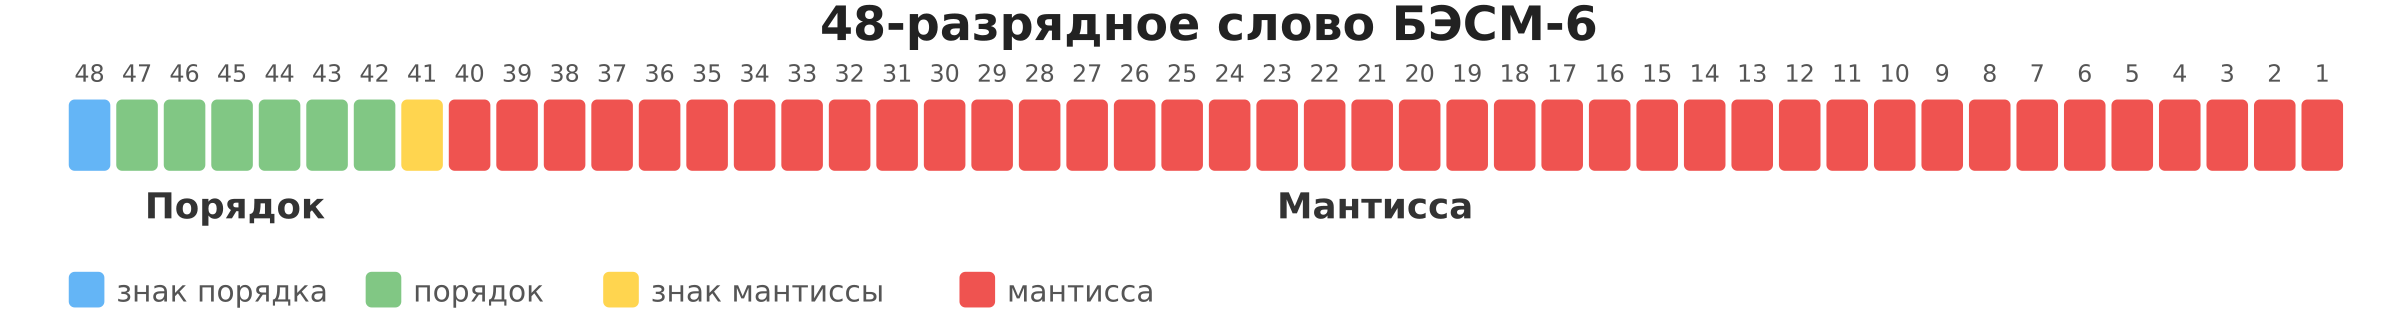
\includegraphics[width=0.85\textwidth]{48-bit.png}
\caption{Формат 48-разрядного машинного слова: знак порядка, шесть разрядов порядка, знак мантиссы и 40~разрядов мантиссы~\cite{saltykov}.}
\end{figure}

В~модели времени \textit{original} длительности рассчитываются по выполненным командам и обращениям к~устройствам с~учётом таблиц из~\cite{saltykov}. Одинаковая последовательность операций даёт одинаковое модельное время независимо от быстродействия хоста. Два эмпирических коэффициента подобраны по двум показателям одного опубликованного прогона Whetstone~\cite{whetstone,se}: сумме времён секций и сумме секций N5 и N8. Опорный прогон также выполнен на модели, а~не на физической машине. Для математических функций приняты оценочные длительности, в~частности 60~мкс для вычисления экспоненты.

Точность учёта времени следует отличать от достоверности принятых длительностей операций. Модель суммирует время воспроизводимо, однако исходные длительности известны приближённо. Поэтому абсолютные значения рассматриваются как оценки порядка величины. Настройка по Whetstone не является независимой проверкой соответствия времени действующей советской ЭВМ.

\subsection{Тестовые программы}

Набор включает перцептрон~\cite{rosenblatt}, метод $k$ ближайших соседей~\cite{cover}, метод $k$-средних~\cite{lloyd}, наивный байесовский классификатор~\cite{domingos}, решающий пень~\cite{holte}, генетический алгоритм~\cite{holland}, имитацию отжига~\cite{kirkpatrick}, Q-обучение~\cite{watkins}, поиск A$^*$~\cite{hart}, многослойный перцептрон~\cite{rumelhart} и поиск мата в~один ход в~упрощённой минишахматной модели~\cite{shannon}. Для десяти алгоритмов сформированы по четыре размера задачи, для многослойного перцептрона сохранена сеть 2--2--1 на четырёх примерах XOR. Всего проверен 41~вариант; итоговое сравнение производительности использует десять больших вариантов и контрольный многослойный перцептрон (табл.~1).

Данные формируются короткими циклами по фиксированным правилам, без развёртывания в~тысячи присваиваний. При увеличении размеров структура исходного текста не меняется. Программы детерминированы. В~тестах с~генератором используется одна последовательность $x \leftarrow (75x + 74) \bmod 65\,537$ с~начальным значением 12~345. Реализации на Python воспроизводят логику и порядок обхода данных и используют только стандартную библиотеку; для вещественных массивов применяются значения типа \texttt{float}.

Размеры выбраны с~учётом памяти БЭСМ-6 и достаточной длительности счёта, а~не равенства числа команд. Для каждой программы параметры одинаковы на сравниваемых платформах. Использованы синтетические нагрузки с~фиксированными бюджетами обучения и поиска; увеличение числа эпох или поколений не означает улучшения качества решения. Наибольший загруженный образ программы с~данными и библиотеками занимает 17~806 слов, или около 104~КиБ; это не оценка пикового рабочего пространства транслятора.

У~отжига увеличены размерность квадратичной целевой функции и число шагов. Положительная температура задаётся гиперболическим расписанием от значения, близкого к~5, до 0,1. В~минишахматном тесте увеличивается корпус разных допустимых позиций, а~не доска и не глубина поиска. Сохраняется упрощение исходного примера: чёрный король рассматривает четыре ортогональных хода; результаты не относятся к~полным правилам шахмат.

\begin{table}[!ht]\small\tabcolsep=4pt
\noindent\textbf{Таблица~1}\ \ Итоговые размеры задач и число команд вычислительного участка без печати\par\vspace{4pt}
\centering
\begin{tabular}{|c|l|l|c|}
\hline
\textnumero & \multicolumn{1}{c|}{Программа} & \multicolumn{1}{c|}{Размер экземпляра задачи} & \hd{Команд\\счёта, млн} \\
\hline
1 & Перцептрон & \hl{512 примеров, 24 признака,\\100 эпох} & 89,860 \\ \hline
2 & \hl{Метод $k$ ближайших\\соседей} & \hl{1024 примера, 12 признаков,\\128 запросов, $k=3$} & 85,563 \\ \hline
3 & Метод $k$-средних & \hl{512 точек, 16 признаков,\\8 кластеров, 20 итераций} & 99,935 \\ \hline
4 & \hl{Наивный байесовский\\классификатор} & \hl{256 примеров, 16 признаков,\\8 классов, 8192 запроса} & 73,036 \\ \hline
5 & Решающий пень & \hl{1024 примера, 1023 порога,\\2 направления} & 82,844 \\ \hline
6 & Генетический алгоритм & \hl{Популяция 512, 1024 поколения,\\целые числа от 0 до 1023} & 164,217 \\ \hline
7 & Имитация отжига & 64 координаты, 30~000 шагов & 48,092 \\ \hline
8 & Q-обучение & \hl{128 состояний, 4000 эпизодов,\\до 512 шагов, 2 действия} & 145,228 \\ \hline
9 & Поиск A$^*$ & Сетка $45\times45$, 2025 узлов & 67,789 \\ \hline
10 & \hl{Многослойный\\перцептрон} & \hl{Сеть 2--2--1, 2000 эпох,\\4 примера XOR} & 1,336 \\ \hline
11 & Минишахматы & Корпус из 2048 позиций & 79,797 \\ \hline
\end{tabular}
\end{table}

\subsection{Измерение времени в модели БЭСМ-6}

Полное модельное время разделяется по наблюдаемым границам исполнения. Подготовка начинается с~исполнения монитора и заканчивается перед первой командой программы по адресу \texttt{01000}, указанному в~карте загрузки. Она включает работу монитора, трансляцию, листинг, подключение библиотек и размещение программы. Счёт измеряется от входа в~программу до первого вызова процедуры форматированного вывода \texttt{BCDWRIT*}. Во всех вариантах результаты печатаются только после окончания вычислений. Оставшийся интервал включает форматирование, вывод и завершение задания.

В~счёт включены инициализация и генерация данных, выполнение алгоритма и формирование контрольных итогов. Счётчики не изменяют гостевую память и поток команд. На каждой границе читается тот же объект статистической модели времени, который формирует показатель \texttt{statisticalModelSeconds}; отдельная сумма условных тактов профайлера вместо него не используется. Подготовка, счёт и заключительный интервал в~сумме дают полное модельное время. Измеренное на хосте время работы эмулятора в~это сравнение не входит.

Для ускорения серии отключено ожидание, ограничивающее скорость эмуляции темпом БЭСМ-6, но сохранён тот же алгоритм расчёта модельного времени. На Linux выполнено парное сравнение с~обычным режимом \textit{original} для одиннадцати малых вариантов и большого варианта Q-обучения. Во всех 12~парах точно совпали модельное время, число команд, печатный вывод и SHA-256 конечной памяти. Это проверка измерительного стенда, а~не точности оценки времени советской ЭВМ.

Вычитание времени пустого задания не применяется: его трансляция и загрузка не равны подготовке исследуемой программы. Дифференциальная оценка по повторениям, использовавшаяся в~предварительной короткой серии, также не переносится на новые варианты. В~новой серии границы измеряются непосредственно, а~нагрузка увеличивается параметрами самой задачи.

\subsection{Измерение времени на современных платформах}

Все окончательные прогоны выполнены на одном Linux-компьютере: Intel Xeon E5-2680 v3 (базовая частота 2,50~ГГц), CPython 3.12.7, GNU Fortran 13.2.1, .NET 8.0.21. Замеры современных реализаций выполнялись последовательно, отдельно от функциональных проверок; Python и дочерние процессы Фортрана закреплены за одним логическим процессором. Частота не фиксировалась, поэтому результаты характеризуют указанную конфигурацию, а~не гарантированную частоту выполнения.

В~Python измеряется процессорное время функции с~помощью \texttt{process\_time\_ns}. Подготовка исходного текста на Фортране в~этот участок не входит. В~нативном коде используется \texttt{CPU\_TIME}. Число вызовов функции выбирается так, чтобы серия занимала около 0,15~с или больше; приводится медиана пяти серий. Повторение используется только для разрешения таймера и не изменяет размер гостевой задачи.

GNU Fortran получает тот же исходный текст, что и транслятор системы <<Дубна>>. Для измерения счёта главная программа преобразуется в~подпрограмму без печати; отдельно скомпилированный драйвер вызывает её и использует возвращаемый контрольный скаляр. Все измерения Фортрана выполнены с~\mbox{\textit{-O0}}, без межмодульной оптимизации: это не оценка предельного быстродействия компилятора. Для проверки результатов отдельно применялись проверки границ массивов и целочисленного переполнения, отключённые в~измерительной сборке. Полные времена процессов измерены по десяти запускам, время компиляции и связывания Фортрана~--- по трём; для этих показателей используется реальное время хоста, а~не процессорное время ядра.

\subsection{Критерии совпадения результатов}

Для целочисленных итогов и контрольных сумм требовалось точное совпадение. Для вещественного результата $x$ использован допуск $10^{-5}+10^{-7}|x|$ относительно независимого расчёта на Python; выводятся шесть знаков после запятой. Допуск не равен единице последнего печатного разряда и не является оценкой полной численной точности. Мантисса содержит 40~двоичных разрядов в~БЭСМ-6, 53~в~CPython и 24~для \texttt{REAL} GNU Fortran. Для почти равных вероятностей в~наивном Байесе явно задано единое относительное правило ничьей с~порогом $10^{-5}$; в~остальных случаях сохраняется первый элемент при равенстве. Сравниваются проверяемые итоговые значения, а~не все внутренние состояния обучения.

\section{Результаты}

\subsection{Время исполнения}

Результаты новой Linux-серии приведены в~табл.~2. Для одиннадцати итоговых программ подготовка занимает 1,415--4,507~с модельного времени, счёт~--- 2,731--89,014~с, вывод с~завершением~--- 4,979--9,506~мс. В~десяти увеличенных нагрузках доля счёта составляет 91,2--98,0\,\%; у~контрольной сети XOR~--- 58,0\,\%. Таким образом, в~итоговом сравнении вычислений преобладание подготовки устранено увеличением самих задач, а~не повторным запуском короткого тела без изменения данных.

\begin{figure}[!ht]
\centering
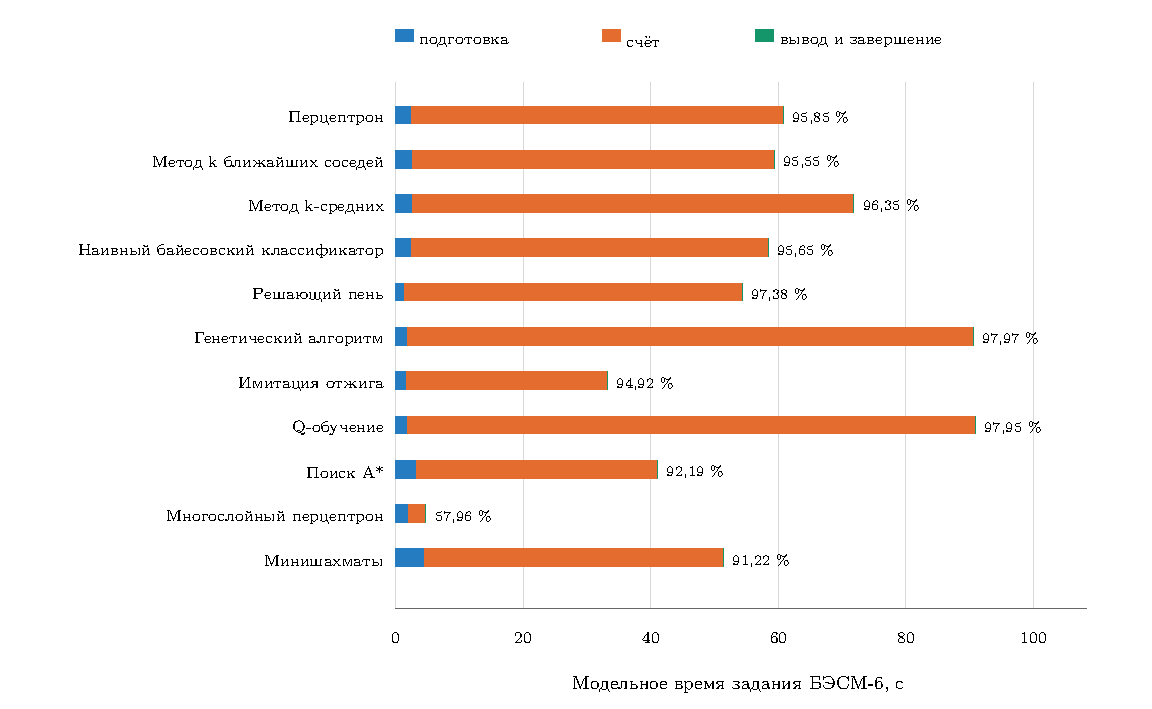
\includegraphics[width=0.96\textwidth]{fig-composition-linux.pdf}
\caption{Распределение модельного времени итоговых заданий между подготовкой, счётом и выводом с~завершением. Все данные относятся к~одной Linux-машине; доля счёта указана справа.}
\label{fig:comp}
\end{figure}

Процессорное время функций Python составляет 5,685--571,015~мс, время кода GNU Fortran с~\mbox{\textit{-O0}}~--- 0,523--12,114~мс. Все указанные интервалы счёта включают инициализацию данных и контрольные итоги, но не печать. Загруженные образы увеличенных программ помещаются в~памяти машины.

\begin{table}[!ht]\small\tabcolsep=3pt
\noindent\textbf{Таблица~2}\ \ Времена итоговых программ: модель БЭСМ-6 и процессорное время современных реализаций\par\vspace{4pt}
\centering
\begin{tabular}{|l|r|r|r|r|r|r|}
\hline
\multicolumn{1}{|c|}{Программа} & \hd{БЭСМ-6:\\подготовка, с} & \hd{БЭСМ-6:\\счёт, с} & \hd{Вывод и\\завершение,\\мс} & \hd{CPython:\\счёт, мс} & \hd{Fortran:\\счёт, мс} & \hd{Доля\\счёта,\%} \\
\hline
Перцептрон & 2,518 & 58,242 & 6,622 & 126,707 & 7,652 & 95,85 \\ \hline
\hl{Метод $k$ ближайших\\соседей} & 2,633 & 56,701 & 5,702 & 126,653 & 8,015 & 95,55 \\ \hline
Метод $k$-средних & 2,612 & 69,232 & 9,506 & 102,179 & 5,291 & 96,35 \\ \hline
\hl{Наивный байесовский\\классификатор} & 2,534 & 55,853 & 6,568 & 94,208 & 5,763 & 95,65 \\ \hline
Решающий пень & 1,415 & 52,890 & 5,819 & 242,145 & 5,871 & 97,38 \\ \hline
Генетический алгоритм & 1,832 & 88,684 & 5,882 & 196,457 & 7,003 & 97,97 \\ \hline
Имитация отжига & 1,677 & 31,509 & 8,299 & 152,404 & 7,897 & 94,92 \\ \hline
Q-обучение & 1,857 & 89,014 & 6,736 & 571,015 & 12,114 & 97,95 \\ \hline
Поиск A$^*$ & 3,199 & 37,837 & 4,979 & 111,004 & 9,271 & 92,19 \\ \hline
\hl{Многослойный\\перцептрон} & 1,973 & 2,731 & 7,703 & 5,685 & 0,523 & 57,96 \\ \hline
Минишахматы & 4,507 & 46,896 & 5,034 & 98,527 & 4,079 & 91,22 \\ \hline
\end{tabular}
\par\smallskip\noindent{\footnotesize Для БЭСМ-6 показано модельное время; для CPython и GNU Fortran~--- измеренное процессорное время. Все измерения Фортрана выполнены с~\mbox{-O0}. Доля счёта относится к~полному модельному времени задания.}
\end{table}

\subsection{Отношения времён}

Модельное время счёта превышает время CPython в~156--678~раз (медиана около 451), время кода GNU Fortran с~\mbox{\textit{-O0}}~--- в~$3{,}99\cdot10^3$--$1{,}31\cdot10^4$ раза (медиана около $7{,}61\cdot10^3$). Отношения рассчитаны по неокруглённым исходным временам, поэтому деление округлённых ячеек таблицы~2 может дать немного другие значения.

\begin{figure}[!ht]
\centering
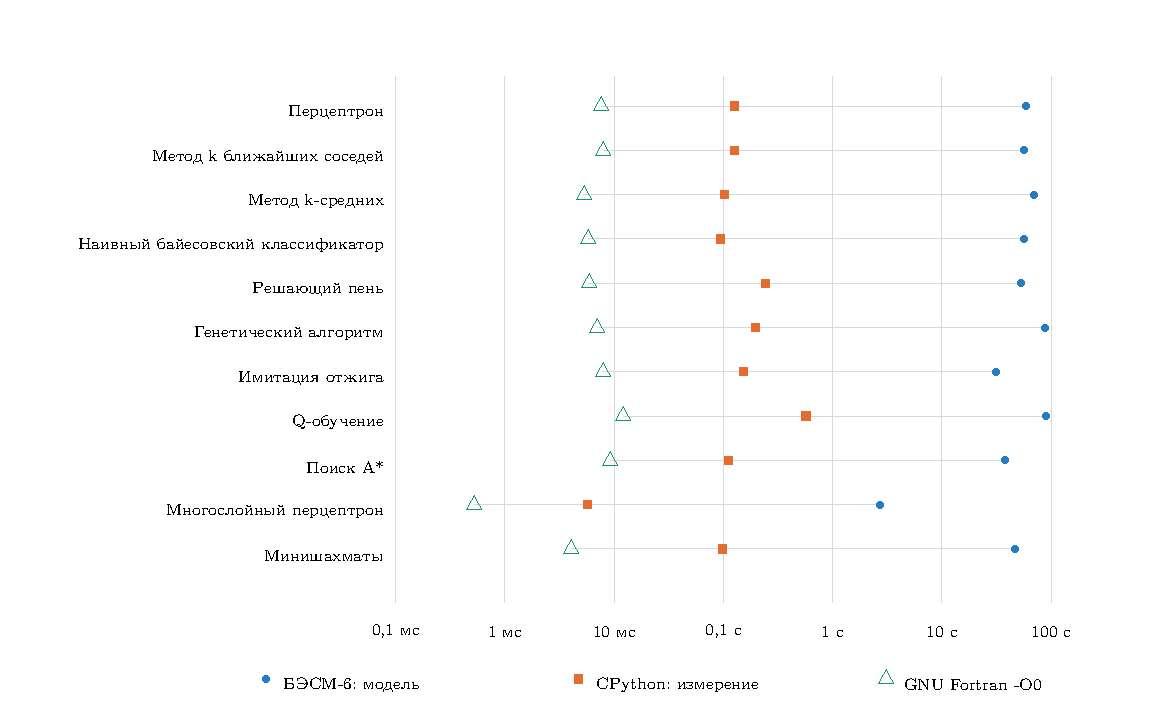
\includegraphics[width=0.96\textwidth]{fig-compute-linux.pdf}
\caption{Время счёта итоговых задач на логарифмической шкале. Для БЭСМ-6 показана модельная оценка, для CPython и GNU Fortran~--- измеренное процессорное время на одном Linux-хосте.}
\label{fig:compute}
\end{figure}

\begin{table}[!ht]\small\tabcolsep=4pt
\noindent\textbf{Таблица~3}\ \ Отношения времён счёта и отдельные затраты современного запуска\par\vspace{4pt}
\centering
\begin{tabular}{|l|c|c|c|c|c|c|}
\hline
 & \multicolumn{3}{c|}{Отношение времён счёта} & \multicolumn{3}{c|}{Реальное время хоста, мс} \\
\cline{2-7}
\multicolumn{1}{|c|}{Программа} & \hd{БЭСМ-6 /\\CPython} & \hd{БЭСМ-6 /\\Fortran} & \hd{CPython /\\Fortran} & \hd{Процесс\\CPython} & \hd{Процесс\\Fortran} & \hd{Компиляция\\Fortran} \\
\hline
Перцептрон & 460 & 7~611 & 16,6 & 171,774 & 8,625 & 48,008 \\ \hline
\hl{Метод $k$ ближайших\\соседей} & 448 & 7~074 & 15,8 & 172,203 & 8,943 & 48,003 \\ \hline
Метод $k$-средних & 678 & 13~084 & 19,3 & 147,592 & 6,213 & 49,136 \\ \hline
\hl{Наивный байесовский\\классификатор} & 593 & 9~691 & 16,3 & 136,650 & 6,792 & 50,116 \\ \hline
Решающий пень & 218 & 9~009 & 41,2 & 292,556 & 6,729 & 45,646 \\ \hline
Генетический алгоритм & 451 & 12~664 & 28,1 & 249,645 & 9,461 & 48,229 \\ \hline
Имитация отжига & 207 & 3~990 & 19,3 & 202,659 & 8,810 & 47,251 \\ \hline
Q-обучение & 156 & 7~348 & 47,1 & 616,148 & 13,070 & 47,815 \\ \hline
Поиск A$^*$ & 341 & 4~081 & 12,0 & 158,899 & 10,162 & 48,434 \\ \hline
\hl{Многослойный\\перцептрон} & 480 & 5~226 & 10,9 & 54,896 & 1,429 & 47,834 \\ \hline
Минишахматы & 476 & 11~497 & 24,2 & 147,762 & 4,965 & 55,025 \\ \hline
\end{tabular}
\par\smallskip\noindent{\footnotesize Время процесса Фортрана относится к~уже скомпилированной программе и не включает компиляцию. Время компиляции включает связывание. Эти показатели измерены отдельно и не выдаются за одинаковый полный цикл подготовки задания на всех платформах.}
\end{table}

Полные времена современных процессов составляют 54,896--616,148~мс для Python и 1,429--13,070~мс для Фортрана. Компиляция и связывание Фортрана занимают отдельно 45,646--55,025~мс. Отношение времени процесса к~времени счёта зависит от нагрузки, поэтому стоимость запуска нельзя представлять как универсальный коэффициент ускорения языка.

Для десяти серий увеличение размеров меняет соотношение подготовки и счёта на противоположное (рис.~\ref{fig:scaling}). Например, в~новой малой задаче перцептрона счёт составляет около 0,013~с, а~в~большой~--- 58,242~с; подготовка возрастает гораздо слабее. Это не означает, что трансляция стала быстрее: уменьшается её доля в~полном времени. Время подготовки может расти из-за констант размеров и размещения данных, даже если число строк программы не меняется.

\begin{figure}[!ht]
\centering
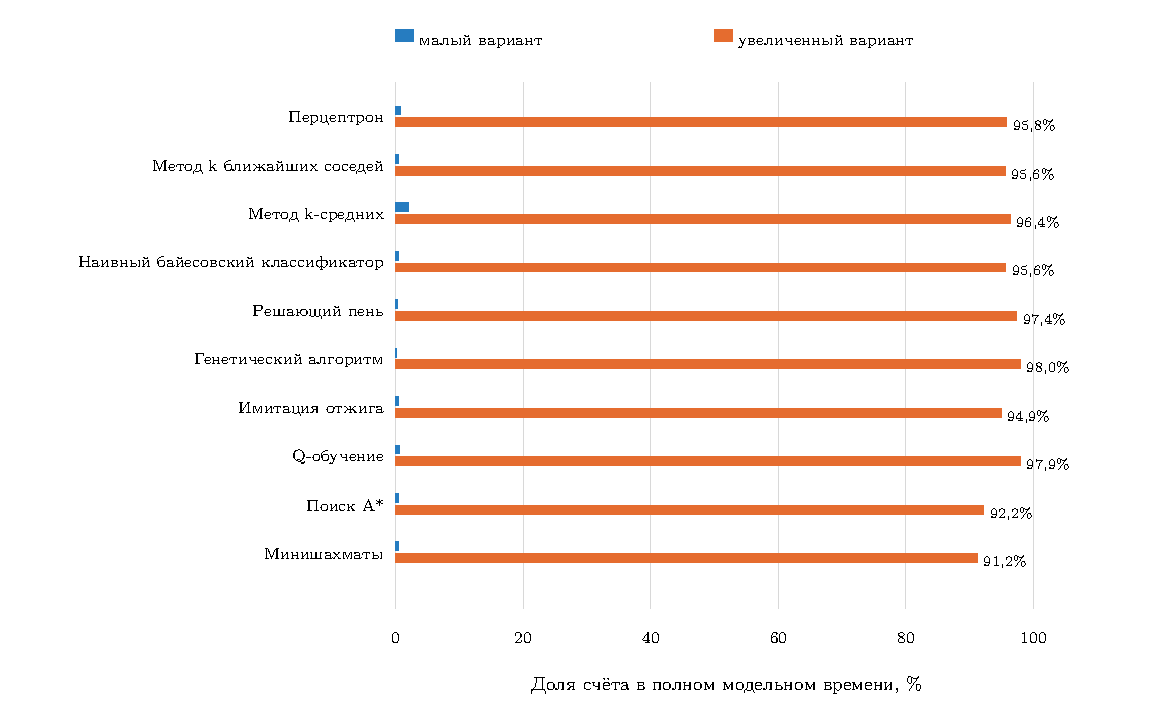
\includegraphics[width=0.96\textwidth]{fig-scaling-linux.pdf}
\caption{Доля счёта для малых и увеличенных вариантов десяти алгоритмов. Показаны крайние размеры каждой серии; все значения получены на одном Linux-хосте.}
\label{fig:scaling}
\end{figure}

\subsection{Совпадение результатов}

Для всех 41~варианта результаты БЭСМ.NET и GNU Fortran согласовались с~независимым расчётом на Python по принятым критериям. Контролировались число верных классификаций и итог весов перцептрона, суммы предсказаний kNN и Байеса, центры и состав кластеров, порог и число ошибок пня, приспособленность популяции, значения целевой функции отжига, политика и сумма Q-таблицы, длина и контрольная сумма пути A$^*$, число ходов и матов в~корпусе минишахматных позиций. Совпадение этих итогов не является доказательством равенства всех промежуточных состояний.

Для многослойного перцептрона проверены все четыре выхода и сумма квадратов ошибок. Значения согласуются с~приблизительными выходами 0,002870; 0,996934; 0,996904; 0,004670 и ошибкой $4{,}90\cdot10^{-5}$. Проверка служит контролем сопоставимости реализаций, а~не общей верификацией процессора или полной численной устойчивости обучения.

\subsection{Перекрёстная проверка}

Все 41~вариант выполнены на SIMH~\cite{simh} под управлением ОС <<Диспак>>. В~основной проверке использована карта \texttt{*FORTRAN}, выбирающая Фортран-Дубна, как и в~БЭСМ.NET. Тело программы совпадает с~телом, передаваемым GNU Fortran. Все контрольные результаты согласовались с~принятыми допусками. Начальная загрузка ОС и физическая модель SIMH отличаются от hosted-исполнения БЭСМ.NET; времена этих двух моделей в~таблицах не смешиваются.

Отдельная серия с~картой \texttt{*FTN} использовала другой транслятор~--- Фортран-ГДР от 10.06.84. В~ней совпали 27~вариантов, а~14~вариантов перцептрона, kNN, Байеса и A$^*$ дали иные результаты. Смена только управляющей карты на \texttt{*FORTRAN} устранила эти расхождения без изменения алгоритмов. Дополнительные малые тесты подтвердили генератор чисел, целочисленную степень, простой поиск минимума и контроль исходных массивов. Причина расхождений в~связке Фортран-ГДР/SIMH без анализа машинного кода не установлена; приписывать их одному эмулятору или одному компилятору преждевременно. Листинги обеих серий сохранены отдельно.

\section{Обсуждение}
\label{sec:discussion}

Увеличение задач позволило сравнивать вычислительные участки, а~не преимущественно подготовку заданий. Полученные отношения характеризуют сочетание выбранных программ, разрядностей, компиляторов и настроек. Они не являются универсальной оценкой быстродействия языка, чистого аппаратного прогресса или скорости самого эмулятора. Особенно важно, что нативный Фортран измерен без оптимизации.

Оценка многослойного перцептрона зависит от принятой длительности экспоненты: 24~012 обращений при 60~мкс и коэффициентах калибровки 1,769 и 0,671 дают около 1,71~с из 2,731~с счёта. Темп, рассчитанный по числу команд вычислительного участка, составляет примерно 1,31--1,85~млн команд в~секунду для десяти больших задач и 0,49~млн для сети XOR. Это следствие принятой временной модели и состава команд, а~не независимая проверка быстродействия советской ЭВМ~\cite{saltykov}.

Основные ограничения следующие. Время выполнения на советской ЭВМ рассчитано, а~не измерено на действующей БЭСМ-6; его абсолютная погрешность не установлена. Синтетические задачи и фиксированные бюджеты выбраны для измерения нагрузки, а~не для оценки практического качества ИИ. Наибольшие размеры отобраны после предварительного исследования времени и памяти, поэтому высокая доля счёта не должна представляться независимым универсальным свойством алгоритмов. Проверяются итоговые значения, а~не вся численная траектория. Современные измерения выполнены на одном хосте, с~одной версией CPython и GNU Fortran; частота процессора не зафиксирована. Расхождения дополнительной серии Фортран-ГДР остаются ограничением переносимости.

\section{Заключение}

Выполнена новая серия из 41~варианта на одной Linux-машине. Инструментальные границы позволили отделить подготовку задания БЭСМ-6 от счёта и заключительного вывода. Для десяти увеличенных задач счёт занимает 91,2--98,0\,\% полного модельного времени; подготовка не исчезает, но перестаёт определять результат сравнения. Контрольная сеть XOR имеет долю счёта около 58\,\%.

В~итоговом наборе модельное время счёта превышает процессорное время CPython в~156--678~раз, кода GNU Fortran с~\mbox{\textit{-O0}}~--- примерно в~4--13~тысяч раз. Эти отношения относятся к~указанным реализациям и модели задержек. Они не измеряют скорость эмулятора и не задают точность восстановления времени настоящей машины.

Все 41~вариант согласовались по контрольным результатам между БЭСМ.NET, Python и GNU Fortran, а~также с~SIMH при выборе Фортрана-Дубна. Отдельно зафиксированы расхождения серии с~Фортраном-ГДР. Исходные тексты, параметры, контрольные суммы, измерительные серии и листинги доступны в~репозитории~\cite{besm6net}; материалы новой Linux-серии отделены от архивных малых тестов.

\section*{\protect\rmfamily Приложение}

\subsection*{\protect\rmfamily П.1\ \ Материалы и пример запуска}

Материалы новой Linux-серии размещены в~репозитории~\cite{besm6net}. Базовый код модели соответствует коммиту \texttt{737349e}; новые сценарии и задания сопровождаются контрольными суммами исходников. Доступны следующие материалы:
\begin{itemize}\raggedright\itemsep=0pt\parskip=0pt
\item задания всех размеров~--- каталог \texttt{examples/ai/scaled/};
\item генерация задач и независимые реализации~--- \texttt{tools/ai\_scaling\_cases.py};
\item измерительный стенд~--- \texttt{tools/AiScalingProbe/};
\item прогоны модели~--- \texttt{tools/benchmark\_ai\_scaling.py};
\item современные измерения~--- \texttt{tools/benchmark\_ai\_scaling\_host.py};
\item проверки GNU Fortran и SIMH~--- сценарии \texttt{tools/check\_ai\_scaling\_native.py} и \texttt{tools/check\_ai\_scaling\_simh.py};
\item числовые серии, параметры и итоговые проверки~--- каталог \texttt{reports/ai-scaling-linux-2026-11-23/}; сводная таблица~--- \texttt{reports/ai-comparison.json}. Полные консольные выводы и листинги хранятся отдельно от Git.
\end{itemize}

Пример запуска опубликованного задания в~обычном режиме модели:

{\small
\begin{verbatim}
dotnet src/Besm6.Cli/bin/Release/net8.0/besm6.dll run \
    examples/ai/scaled/perceptron-l3.dub --speed original --stats \
    --guest-clock --no-wall-clock
\end{verbatim}
}

\noindent Режим \texttt{--speed original} включает временную модель БЭСМ-6 и ограничение темпа. Ключ \texttt{--stats} выводит общие счётчики. Параметр \texttt{--guest-clock} включает модельные часы, а~\texttt{--no-wall-clock} фиксирует дату.

Границы подготовки, счёта и вывода измеряются отдельным стендом; общая статистика CLI сама по себе их не разделяет.

\subsection*{\protect\rmfamily П.2\ \ Условия дополнительной проверки}

SIMH собран из коммита \texttt{698dc8a1}; для ОС <<Диспак>> использованы опубликованные образы \texttt{sbor2048.bin}, \texttt{sbor2053.bin}, \texttt{svs2048.bin} и \texttt{alt2048.bin}. Контрольные суммы образов и конфигурации запуска сохранены с~результатами. Каждый запуск использует отдельные копии дисков, чтобы изменения ОС не переходили к~следующему тесту. В~основной серии выбирается \texttt{*FORTRAN}; серия \texttt{*FTN} хранится как отдельная проверка переносимости.

Все 41~задание завершаются \texttt{STOP} в~БЭСМ.NET, GNU Fortran и основной серии SIMH. Для измерительного стенда сохранены 12~пар обычного и ускоренного исполнения с~проверкой модельного времени, счётчиков, вывода и конечной памяти. Современные тайминги сопровождаются исходными пятью сериями, числом повторений, десятью временами процессов и тремя временами компиляции. Архивные малые тесты и прежние измерения на Windows не включены в~числа новой Linux-серии.

\section*{\protect\rmfamily Вклад авторов}
\noindent\textbf{А.\,В.~Солопий}~--- разработка эмулятора, тестирование, проведение запусков и расчётов.

\smallskip\noindent
\textbf{Р.\,Ф.~Гибадуллин}~--- вычитка, редактирование и верификация.

% Конфликт интересов и финансирование: заполнить после подтверждения авторами.

{\small\frenchspacing
  \begin{thebibliography}{99}
\bibitem{bre}
БЭСМ-6~// Большая российская энциклопедия. \texttt{https://bigenc.ru/c/besm-6-4f8e4d} (дата обращения: 18.11.2026).
\bibitem{dubna}
{\it Говорун Н.\,Н., Силин И.\,Н. и~др.} Мониторная система <<Дубна>> для ЭВМ БЭСМ-6~// Тр. второй Всесоюзной конф. по программированию.~--- Новосибирск: ВЦ СО АН СССР, 1970.
\bibitem{saltykov}
{\it Салтыков А.\,И., Макаренко Г.\,И.} Программирование на языке фортран~/ Под ред. Н.\,Н.~Говоруна.~--- М.: Наука, 1976. 256~с.
\bibitem{besm6net}
besm6.net~--- эмулятор ЭВМ БЭСМ-6. \texttt{https://github.com/EntityFX/besm6.net} (дата обращения: 18.11.2026).
\bibitem{whetstone}
{\it Curnow H.\,J., Wichmann B.\,A.} A~synthetic benchmark~// Comput.~J., 1976. Vol.~19. No.\,1. P.~43--49. doi: 10.1093/comjnl/19.1.43.
\bibitem{se}
How to compute performance of a CPU in FLOPS~// Retrocomputing Stack Exchange, 2017. \texttt{https://retrocomputing.stackexchange.com/\allowbreak questions/3267/\allowbreak how-to-compute-performance-of-a-cpu-in-flops} (дата обращения: 18.11.2026).
\bibitem{rosenblatt}
{\it Rosenblatt F.} The perceptron: A~probabilistic model for information storage and organization in the brain~// Psychol. Rev., 1958. Vol.~65. No.\,6. P.~386--408. doi: 10.1037/h0042519.
\bibitem{cover}
{\it Cover T.\,M., Hart P.\,E.} Nearest neighbor pattern classification~// IEEE T. Inform. Theory, 1967. Vol.~13. No.\,1. P.~21--27. doi: 10.1109/TIT.1967.1053964.
\bibitem{lloyd}
{\it Lloyd S.\,P.} Least squares quantization in PCM~// IEEE T. Inform. Theory, 1982. Vol.~28. No.\,2. P.~129--137. doi: 10.1109/TIT.1982.1056489.
\bibitem{domingos}
{\it Domingos P., Pazzani M.} On the optimality of the simple Bayesian classifier under zero-one loss~// Mach. Learn., 1997. Vol.~29. P.~103--130. doi: 10.1023/A:1007413511361.
\bibitem{holte}
{\it Holte R.\,C.} Very simple classification rules perform well on most commonly used datasets~// Mach. Learn., 1993. Vol.~11. P.~63--90. doi: 10.1023/A:1022631118932.
\bibitem{holland}
{\it Holland J.\,H.} Adaptation in natural and artificial systems.~--- Ann Arbor, MI, USA: University of Michigan Press, 1975.
\bibitem{kirkpatrick}
{\it Kirkpatrick S., Gelatt C.\,D., Vecchi M.\,P.} Optimization by simulated annealing~// Science, 1983. Vol.~220. No.\,4598. P.~671--680. doi: 10.1126/science.220.4598.671.
\bibitem{watkins}
{\it Watkins C.\,J.\,C.\,H., Dayan P.} Q-learning~// Mach. Learn., 1992. Vol.~8. P.~279--292. doi: 10.1007/BF00992698.
\bibitem{hart}
{\it Hart P.\,E., Nilsson N.\,J., Raphael B.} A~formal basis for the heuristic determination of minimum cost paths~// IEEE T. Syst. Sci. Cyb., 1968. Vol.~4. No.\,2. P.~100--107. doi: 10.1109/TSSC.1968.300136.
\bibitem{rumelhart}
{\it Rumelhart D.\,E., Hinton G.\,E., Williams R.\,J.} Learning representations by back-propagating errors~// Nature, 1986. Vol.~323. P.~533--536. doi: 10.1038/323533a0.
\bibitem{shannon}
{\it Shannon C.\,E.} Programming a computer for playing chess~// Philos. Mag., 1950. Vol.~41. No.\,314. P.~256--275. doi: 10.1080/14786445008521796.
\bibitem{simh}
SIMH. \texttt{https://github.com/simh/simh} (дата обращения: 18.11.2026).
\end{thebibliography}
}

\clearpage
\selectlanguage{english}

\def\tit{SEPARATE MEASUREMENT OF~TRANSLATION, COMPUTATION, AND~OUTPUT TIMES IN~A~SOFTWARE MODEL OF~THE~BESM-6 COMPUTER: A~CASE STUDY OF~ARTIFICIAL INTELLIGENCE ALGORITHMS}

\def\titkol{Separate measurement of translation, computation, and output times in a software model of the BESM-6 computer}

\def\aut{A.\,V.~Solopiy and R.\,F.~Gibadullin}

\def\autkol{A.\,V.~Solopiy and R.\,F.~Gibadullin}

\titel{\tit}{\aut}{\autkol}{\titkol}

\noindent
Kazan National Research Technical University named after A.N.~Tupolev-KAI, 10~K.~Marx Str., Kazan 420111, Russian Federation

\Abste{Classical artificial intelligence algorithms are evaluated using a~software model of the Soviet BESM-6 computer and modern Python and Fortran implementations. Four problem sizes are prepared for each of ten algorithms, with a~multilayer perceptron included as a~separate control. Instruction counters and model clocks separate job preparation, computation, and output with termination. Preparation dominates the small workloads because of their limited computational volume, not because of an inherent property of artificial intelligence algorithms. In the ten enlarged workloads, computation accounts for 91.2--98.0\% of total model time. All experiments are run on one Linux computer. BESM-6 execution time is estimated using the adopted timing model, rather than measured as emulator speed; CPython and GNU Fortran kernel times are measured as process CPU time. In the final set of eleven programs, model computation time exceeds CPython time by factors of 156--678 and unoptimized GNU Fortran time by approximately 4--13 thousand. Integer control results agree exactly, and real-valued results agree within the specified tolerance despite the different 48-, 32-, and 64-bit number formats. All 41 variants are additionally checked using the independent SIMH emulator with the Dubna Fortran translator.}

\KWE{BESM-6; computer emulation; timing model; performance measurement; Fortran; Python; artificial intelligence algorithms}

\renewcommand{\refname}{\protect\rmfamily References}

{\small\frenchspacing
  \begin{thebibliography}{99}
\bibitem{bre-e}
BESM-6. \textit{Bol'shaya rossiyskaya entsiklopediya} [Great Russian Encyclopedia]. Available at: \texttt{https://bigenc.ru/c/besm-6-4f8e4d} (accessed November~18, 2026).
\bibitem{dubna-e}
Govorun, N.\,N., I.\,N.~Silin, et~al. 1970. Monitornaya sistema <<Dubna>> dlya EVM BESM-6 [The Dubna monitor system for the BESM-6 computer]. \textit{Trudy vtoroy Vsesoyuznoy konferentsii po programmirovaniyu} [2nd All-Union Conference on Programming Proceedings]. Novosibirsk.
\bibitem{saltykov-e}
Saltykov, A.\,I., and G.\,I.~Makarenko. 1976. \textit{Programmirovanie na yazyke fortran} [Programming in Fortran]. Ed. N.\,N.~Govorun. Moscow: Nauka. 256~p.
\bibitem{besm6net-e}
besm6.net~--- emulyator EVM BESM-6 [besm6.net: An~emulator of the BESM-6 computer]. Available at: \texttt{https://github.com/EntityFX/besm6.net} (accessed November~18, 2026).
\bibitem{whetstone-e}
Curnow, H.\,J., and B.\,A.~Wichmann. 1976. A~synthetic benchmark. \textit{Comput.~J.} 19(1):43--49. doi: 10.1093/comjnl/19.1.43.
\bibitem{se-e}
How to compute performance of a CPU in FLOPS. 2017. \textit{Retrocomputing Stack Exchange}. Available at: \texttt{https://retrocomputing.stackexchange.com/\allowbreak questions/3267/\allowbreak how-to-compute-performance-of-a-cpu-in-flops} (accessed November~18, 2026).
\bibitem{rosenblatt-e}
Rosenblatt, F. 1958. The perceptron: A~probabilistic model for information storage and organization in the brain. \textit{Psychol. Rev.} 65(6):386--408. doi: 10.1037/h0042519.
\bibitem{cover-e}
Cover, T.\,M., and P.\,E.~Hart. 1967. Nearest neighbor pattern classification. \textit{IEEE T. Inform. Theory} 13(1):21--27. doi: 10.1109/TIT.1967.1053964.
\bibitem{lloyd-e}
Lloyd, S.\,P. 1982. Least squares quantization in PCM. \textit{IEEE T. Inform. Theory} 28(2):129--137. doi: 10.1109/TIT.1982.1056489.
\bibitem{domingos-e}
Domingos, P., and M.~Pazzani. 1997. On the optimality of the simple Bayesian classifier under zero-one loss. \textit{Mach. Learn.} 29:103--130. doi: 10.1023/A:1007413511361.
\bibitem{holte-e}
Holte, R.\,C. 1993. Very simple classification rules perform well on most commonly used datasets. \textit{Mach. Learn.} 11:63--90. doi: 10.1023/A:1022631118932.
\bibitem{holland-e}
Holland, J.\,H. 1975. \textit{Adaptation in natural and artificial systems}. Ann Arbor, MI: University of Michigan Press.
\bibitem{kirkpatrick-e}
Kirkpatrick, S., C.\,D.~Gelatt, and M.\,P.~Vecchi. 1983. Optimization by simulated annealing. \textit{Science} 220(4598):671--680. doi: 10.1126/science.220.4598.671.
\bibitem{watkins-e}
Watkins, C.\,J.\,C.\,H., and P.~Dayan. 1992. Q-learning. \textit{Mach. Learn.} 8:279--292. doi: 10.1007/BF00992698.
\bibitem{hart-e}
Hart, P.\,E., N.\,J.~Nilsson, and B.~Raphael. 1968. A~formal basis for the heuristic determination of minimum cost paths. \textit{IEEE T. Syst. Sci. Cyb.} 4(2):100--107. doi: 10.1109/TSSC.1968.300136.
\bibitem{rumelhart-e}
Rumelhart, D.\,E., G.\,E.~Hinton, and R.\,J.~Williams. 1986. Learning representations by back-propagating errors. \textit{Nature} 323:533--536. doi: 10.1038/323533a0.
\bibitem{shannon-e}
Shannon, C.\,E. 1950. Programming a computer for playing chess. \textit{Philos. Mag.} 41(314):256--275. doi: 10.1080/14786445008521796.
\bibitem{simh-e}
SIMH. Available at: \texttt{https://github.com/simh/simh} (accessed November~18, 2026).
\end{thebibliography}
}

\Contr
\textbf{Solopiy Artem V.} (b.~1989)~--- assistant lecturer, Department of Computer Systems, Kazan National Research Technical University named after A.N.~Tupolev-KAI, 10~K.~Marx Str., Kazan 420111, Russian Federation; \mbox{artem.solopiy@gmail.com}

\smallskip
\noindent
\textbf{Gibadullin Ruslan F.} (b.~1984)~--- Candidate of Science (PhD) in technology, associate professor, Department of Computer Systems, Kazan National Research Technical University named after A.N.~Tupolev-KAI, 10~K.~Marx Str., Kazan 420111, Russian Federation; \mbox{RFGibadullin@kai.ru}

\selectlanguage{russian}
\section*{\protect\rmfamily Сведения об авторах}\noindent
\textbf{Солопий Артём Валерьевич} (р.~1989)~--- ассистент кафедры компьютерных систем Казанского национального исследовательского технического университета им.\ А.\,Н.~Туполева--КАИ, ул.\ К.\ Маркса, 10, Казань, 420111, Россия; \mbox{artem.solopiy@gmail.com}

\smallskip
\noindent
\textbf{Гибадуллин Руслан Фаршатович} (р.~1984)~--- кандидат технических наук, доцент кафедры компьютерных систем Казанского национального исследовательского технического университета им.\ А.\,Н.~Туполева--КАИ, ул.\ К.\ Маркса, 10, Казань, 420111, Россия; \mbox{RFGibadullin@kai.ru}

\end{document}
